\documentclass[11pt, a4paper]{article}

% =============================================================================
% TALIM — Hackathon Pitch Document
% =============================================================================

% ── Packages ─────────────────────────────────────────────────────────────────
\usepackage[margin=2.2cm, top=2.4cm, bottom=2.4cm]{geometry}
\usepackage[T1]{fontenc}
\usepackage[utf8]{inputenc}
\usepackage{lmodern}
\usepackage[expansion=false]{microtype}
\usepackage{parskip}
\usepackage{titlesec}
\usepackage{enumitem}
\usepackage{booktabs}
\usepackage{tabularx}
\usepackage{array}
\usepackage{xcolor}
\usepackage{graphicx}
\usepackage{hyperref}
\usepackage{fancyhdr}
\usepackage{multicol}
\usepackage{tcolorbox}
\usepackage{amsmath}
\usepackage{setspace}
\usepackage{tikz}
\usetikzlibrary{shapes.geometric, arrows.meta, positioning, calc, fit, backgrounds}

% ── Color Palette (Kashmir-rooted) ───────────────────────────────────────────
\definecolor{ink}{HTML}{1A1A1A}
\definecolor{lapis}{HTML}{1E3A5F}        % deep lapis lazuli — Kashmiri miniature blue
\definecolor{saffron}{HTML}{C7811C}      % kesar / saffron
\definecolor{walnut}{HTML}{5B3A1E}       % walnut wood
\definecolor{paper}{HTML}{FAF6EC}        % aged paper / talim sheet
\definecolor{paperdark}{HTML}{EFE6D2}
\definecolor{muted}{HTML}{6B7280}
\definecolor{accent}{HTML}{B91C1C}
\definecolor{success}{HTML}{15803D}
\definecolor{rule}{HTML}{C7811C}

% ── Hyperref ─────────────────────────────────────────────────────────────────
\hypersetup{
  colorlinks=true,
  linkcolor=lapis,
  urlcolor=saffron,
  citecolor=lapis,
  pdfauthor={Team TALIM},
  pdftitle={TALIM — Digital Apprenticeship for Kashmir's Living Crafts},
}

% ── Typography ───────────────────────────────────────────────────────────────
\titleformat{\section}
  {\Large\bfseries\color{lapis}}
  {\thesection.}{0.6em}{}
  [\vspace{-0.25em}\color{rule}\rule{\linewidth}{1.4pt}]

\titleformat{\subsection}
  {\normalsize\bfseries\color{walnut}}
  {\thesubsection}{0.5em}{}

\titleformat{\subsubsection}
  {\normalsize\itshape\color{muted}}
  {}{0em}{}

\titlespacing{\section}{0pt}{1.6em}{0.6em}
\titlespacing{\subsection}{0pt}{1em}{0.35em}

% ── Header / Footer ──────────────────────────────────────────────────────────
\pagestyle{fancy}
\fancyhf{}
\fancyhead[L]{\small\textbf{\color{lapis}TALIM} \color{muted}— Digital Apprenticeship for Kashmir's Living Crafts}
\fancyhead[R]{\small\color{muted}Hackathon Pitch · 2025}
\fancyfoot[C]{\small\color{muted}\thepage}
\renewcommand{\headrulewidth}{0.4pt}
\renewcommand{\footrulewidth}{0pt}

% ── tcolorbox ────────────────────────────────────────────────────────────────
\tcbuselibrary{skins, breakable}

\newtcolorbox{heroquote}{
  colback=paper, colframe=saffron,
  left=14pt, right=14pt, top=10pt, bottom=10pt,
  arc=2pt, boxrule=1pt, breakable
}

\newtcolorbox{kashmirbox}[1][]{
  colback=paper, colframe=walnut,
  fonttitle=\bfseries\small\color{paper},
  coltitle=paper, colbacktitle=walnut,
  title=#1, attach boxed title to top left={xshift=8pt, yshift=-2pt},
  boxed title style={arc=1pt, boxrule=0pt},
  left=10pt, right=10pt, top=12pt, bottom=8pt,
  arc=2pt, boxrule=0.6pt, breakable
}

\newtcolorbox{insightbox}[1][]{
  colback=paperdark, colframe=lapis,
  fonttitle=\bfseries\small\color{paper},
  coltitle=paper, colbacktitle=lapis,
  title=#1, attach boxed title to top left={xshift=8pt, yshift=-2pt},
  boxed title style={arc=1pt, boxrule=0pt},
  left=10pt, right=10pt, top=12pt, bottom=8pt,
  arc=2pt, boxrule=0.6pt, breakable
}

\newtcolorbox{warnbox}{
  colback=red!4!white, colframe=accent,
  left=10pt, right=10pt, top=8pt, bottom=8pt,
  arc=2pt, breakable
}

\newtcolorbox{statbox}{
  colback=lapis, coltext=paper, colframe=lapis,
  left=12pt, right=12pt, top=10pt, bottom=10pt,
  arc=3pt, breakable
}

\newtcolorbox{uspbox}{
  enhanced, colback=ink, coltext=paper, colframe=saffron,
  borderline west={3pt}{0pt}{saffron},
  left=14pt, right=14pt, top=12pt, bottom=12pt,
  arc=2pt, boxrule=0pt, breakable
}

% ── Lists ────────────────────────────────────────────────────────────────────
\setlist[itemize]{leftmargin=1.3em, itemsep=2pt, topsep=3pt}
\setlist[enumerate]{leftmargin=1.4em, itemsep=2pt, topsep=3pt}

% =============================================================================
\begin{document}
% =============================================================================

% ── Title block ──────────────────────────────────────────────────────────────
\begin{center}
  {\fontsize{40}{44}\selectfont\bfseries\color{lapis} TALIM}\\[2pt]
  {\small\color{saffron}\itshape\textbf{ta'l\u{\i}m}\,\textbar\,Arabic-Kashmiri\,\textbar\,(1) teaching, instruction; (2) the encoded weaving notation invented by Kashmiri masters to pass craft across generations}\\[10pt]
  {\Large\color{walnut}\itshape Digital Apprenticeship for Kashmir's Living Crafts}\\[10pt]
  {\small\color{muted} Hackathon Pitch · NIT Srinagar · Team of 5 · 2025}
\end{center}

\vspace{0.4em}
\noindent\color{rule}\rule{\linewidth}{1.5pt}
\vspace{0.6em}

% ── Opening hero quote ───────────────────────────────────────────────────────
\begin{heroquote}
\centering
\itshape\large\color{walnut}
``A century ago, a Kashmiri master weaver wrote a {\bfseries\color{saffron}talim} \\
so the apprentice could weave a shawl he had never seen. \\[3pt]
Today, that master is dying. The apprentice never came. \\[3pt]
We are writing the {\bfseries\color{saffron}next talim} — \\
the one that teaches anyone, anywhere, in their voice.''
\end{heroquote}

% =============================================================================
\section{One-Sentence Pitch}
% =============================================================================

\begin{uspbox}
\textbf{TALIM is an AI-powered digital apprenticeship platform that captures every Kashmiri master craftsman's lifetime of knowledge in their own voice and language, turns it into an interactive teacher that anyone can learn from, and certifies authentic pieces with a cryptographic Sanad — so the craft outlives the craftsman, the next generation can learn it without leaving home, and every authentic piece pays the artisan, not a middleman.}
\end{uspbox}

\smallskip

We did not invent the idea of encoding a master's knowledge for the next generation. \textbf{Kashmiri masters did, centuries ago, and they called it the {\itshape talim}}. We are simply giving their invention the medium it always deserved.

% =============================================================================
\section{Why This Wins: The USP Nobody Else Can Copy}
% =============================================================================

\begin{kashmirbox}[The Indigenous-Tech Insight]
The {\itshape talim} is not a metaphor. It is a real, documented, centuries-old encoded notation system invented by Kashmiri carpet and shawl weavers. A {\itshape talim-guru} would write a cryptic vertical script — a colour-and-knot code — and an apprentice who had never seen the design could weave it perfectly.\\[4pt]
\textbf{Kashmir invented the world's first source code for craft.} It was paper-based, hand-written, and bound to one workshop. We are not introducing foreign technology to Kashmir. We are upgrading the {\itshape talim} into its inevitable digital form — and we are doing it for {\bfseries every} Kashmiri craft, not just carpets.
\end{kashmirbox}

This single framing gives us five compounding advantages that no generic ``heritage marketplace'' can match:

\begin{enumerate}
  \item \textbf{Cultural authority.} The product is named after, modeled on, and built in service of a Kashmiri tradition. A judge from Srinagar recognises this within ten seconds.
  \item \textbf{A clear, ownable category.} Not ``Etsy for crafts.'' Not ``a heritage app.'' \textit{Digital apprenticeship.} New category, single word, defensible.
  \item \textbf{A teaching focus, not a marketplace focus.} Every competitor is selling. We are \textit{transmitting}. That is the actual problem — without new apprentices, no marketplace can save the craft.
  \item \textbf{A built-in success story.} The talim already proved this model works. We are not asking the jury to bet on a hypothesis; we are asking them to bet on a Kashmiri tradition that has worked for 400 years, now scaled by AI.
  \item \textbf{An unforgeable moat.} The first interview with a living master enters the canonical Kashmiri craft corpus. Every recording is irreplaceable. A competitor starting later cannot interview a master who has died.
\end{enumerate}

\begin{insightbox}[The Brutal One-Liner]
\textbf{Every other team will pitch a product. We are pitching a tradition the jury already believes in, with the technology that finally makes it possible to scale.}
\end{insightbox}

% =============================================================================
\section{The Problem, Stated Plainly}
% =============================================================================

The story starts in a Srinagar workshop, not in a slide deck.

A 72-year-old {\itshape ustaad} of {\itshape sozni} embroidery threads a needle that he has held since he was nine. His hands know a stitch that took thirty years to perfect. His son drives a taxi in Sopore. His grandson is studying for an exam in Bengaluru. Neither of them can sozni a single petal.

The {\itshape ustaad} will pass away in this decade. With him will go a stitch that no museum has, no book has captured, and no algorithm has ever seen.

Multiply this by the master {\itshape Kani} weaver in Kanihama, the {\itshape khatamband} ceiling-maker in Downtown, the {\itshape naqash} painter who layers gold leaf on papier-mâché, the walnut-wood carver in Ishber. Multiply by ten thousand workshops. This is what is happening in Kashmir, right now, this year.

\begin{statbox}
\textbf{The four facts that frame this hackathon:}\\[4pt]
\textbf{1.} Kashmir's craft sector employs \textbf{\textasciitilde 4 lakh artisans} and exports \textbf{\textasciitilde Rs.\ 1{,}600 crore} annually — yet over \textbf{60\%} of ``Kashmiri'' goods sold globally are counterfeits made elsewhere.\\[3pt]
\textbf{2.} The average age of a Kashmiri master craftsman has risen from 36 (1980s) to over \textbf{55 today}. New apprentice enrolment in traditional crafts has fallen by \textbf{more than 50\%} in two decades.\\[3pt]
\textbf{3.} Children of artisans cite three reasons for not entering the craft: \textbf{(a)} it pays poorly because middlemen take 70--85\% of end-buyer value, \textbf{(b)} learning takes 7--12 years of physical apprenticeship that conflicts with formal schooling, \textbf{(c)} no one outside the workshop ever sees their family's name.\\[3pt]
\textbf{4.} Less than \textbf{1\%} of Kashmiri craft businesses have any structured documentation of their own techniques. When the master dies, the technique dies.
\end{statbox}

\subsection{Why existing platforms cannot solve this}

\begin{center}
\small
\begin{tabularx}{\linewidth}{>{\bfseries}lXX}
\toprule
Platform & What it does & Why it fails Kashmir \\
\midrule
Etsy / Amazon Handmade & Sells handmade goods & No verification; floods of counterfeits; no teaching \\
GI Tag (Kashmir Pashmina, etc.) & Legal protection of category names & Protects the {\itshape category}, not individual masters; no learning path \\
YouTube tutorials & Free video content & Random, unstructured, non-Koshur, no certification, no apprentice path \\
Museum archives (INTACH, CDI) & Preserve historical objects & Read-only; not interactive; not in masters' voices \\
Govt.\ skill schemes (PMKVY, etc.) & Train new artisans & Generic curricula; no master-specific knowledge transfer \\
\bottomrule
\end{tabularx}
\end{center}

None of these solve the actual chain: \textit{Master $\to$ Knowledge $\to$ Apprentice $\to$ Income $\to$ Survival of craft.}

% =============================================================================
\section{The Solution: TALIM in Three Pillars}
% =============================================================================

We deliberately reduced the system to \textbf{three pillars}. Anything more is a slide-deck product.

\begin{center}
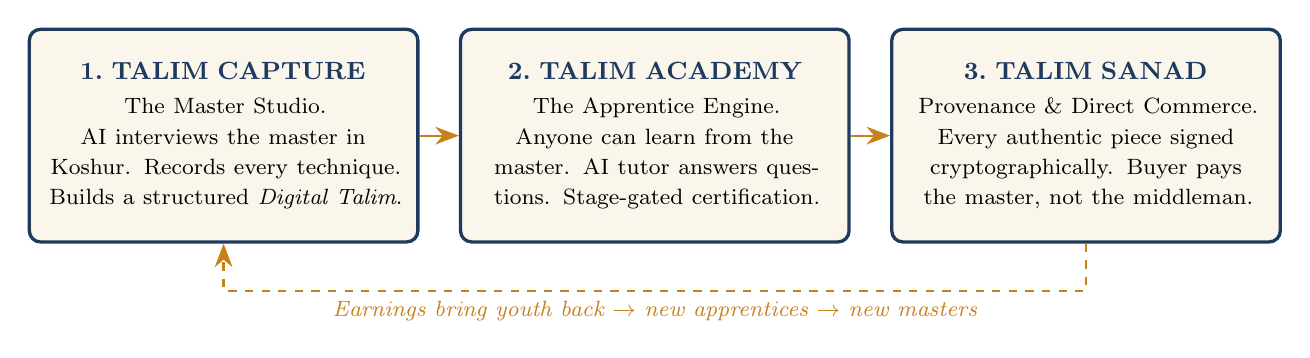
\begin{tikzpicture}[
    node distance=1.4cm and 0.5cm,
    pillar/.style={rectangle, rounded corners=4pt, draw=lapis, very thick, fill=paper, text width=4.7cm, minimum height=2.7cm, align=center, font=\small},
    title/.style={font=\bfseries\color{lapis}},
    flowarrow/.style={-{Stealth[length=3mm]}, thick, color=saffron},
  ]
  \node[pillar] (capture) {\textbf{\color{lapis}1.\ TALIM CAPTURE}\\[3pt]
    \footnotesize The Master Studio.\\
    AI interviews the master in Koshur. Records every technique. Builds a structured \textit{Digital Talim}.};
  \node[pillar, right=of capture] (academy) {\textbf{\color{lapis}2.\ TALIM ACADEMY}\\[3pt]
    \footnotesize The Apprentice Engine.\\
    Anyone can learn from the master. AI tutor answers questions. Stage-gated certification.};
  \node[pillar, right=of academy] (sanad) {\textbf{\color{lapis}3.\ TALIM SANAD}\\[3pt]
    \footnotesize Provenance \& Direct Commerce.\\
    Every authentic piece signed cryptographically. Buyer pays the master, not the middleman.};

  \draw[flowarrow] (capture.east) -- (academy.west);
  \draw[flowarrow] (academy.east) -- (sanad.west);
  \draw[flowarrow, dashed] (sanad.south) -- ++(0,-0.6) -| node[pos=0.25, below, font=\footnotesize\itshape\color{walnut}]{Earnings bring youth back $\to$ new apprentices $\to$ new masters} (capture.south);
\end{tikzpicture}
\end{center}

\subsection{Pillar 1 — TALIM CAPTURE: The Master Studio}

\textbf{Purpose:} Take everything inside a master's head and put it into a permanent, structured, queryable record — \textbf{in their own voice, in Koshur, in a single sitting they can complete on a basic phone}.

\subsubsection{The Master Studio session}

A field facilitator (NIT Srinagar volunteer, CDI student, family member) sits with the master and opens the TALIM Master Studio on a tablet or phone. The session has four passes:

\begin{enumerate}[label=\textbf{Pass \arabic*.}]
  \item \textbf{Lineage \& Identity.} The AI interviewer asks who taught them, where, in what generation. The master speaks freely in Koshur. The system transcribes, translates, and indexes.
  \item \textbf{Technique walkthrough.} The master performs one full technique — say, a single sozni petal. The phone is mounted; voice + video are recorded together. The AI asks structured probes: \textit{``What is this stitch called? What thread count? What needle? What did you adjust just then, and why?''}
  \item \textbf{The decision questions.} The most important pass. The AI asks the questions that no apprentice ever thinks to ask: \textit{``How do you know the wool is good? What will you do if the dye lot is different next month? What mistake did your teacher correct most often?''} This is where tacit knowledge is captured.
  \item \textbf{The talim digitisation.} If the master uses a written {\itshape talim} (carpet/shawl weavers do), it is photographed, OCR-decoded, and stored as machine-readable pattern code linked to the technique.
\end{enumerate}

\subsubsection{What gets produced — the Digital Talim}

The session output is a structured \textbf{Digital Talim Record} with:

\begin{itemize}
  \item Indexed video segments by named technique and tool
  \item Transcribed and translated voice in Koshur, Urdu, English (and on demand: French, Japanese, German for export buyers)
  \item A technique knowledge graph: techniques $\to$ sub-steps $\to$ tools $\to$ materials $\to$ failure modes
  \item Master's lineage and verification metadata
  \item Cryptographic identity (Ed25519 keypair) — this master can now sign Sanads on physical pieces
\end{itemize}

\subsubsection{Knowledge Vulnerability Index}

Every Digital Talim is scored on a {\bfseries Knowledge Vulnerability Index} that combines master's age, technique uniqueness across the corpus, and documentation completeness. A high-vulnerability technique (only one master in the corpus knows it, master is over 70, less than 30 minutes recorded) gets flagged for an emergency follow-up session. This is how we make sure no technique slips through.

\subsection{Pillar 2 — TALIM ACADEMY: The Apprentice Engine}

\textbf{Purpose:} Turn each master's Digital Talim into something a 16-year-old in Anantnag, a design student in Mumbai, or a serious learner in Kyoto can actually \textit{learn from}.

\subsubsection{The learner experience}

A learner enters the Academy and chooses a craft (e.g., Sozni). They see the masters whose Digital Talims are available and pick one. From that moment, the learner has a personal curriculum:

\begin{itemize}
  \item \textbf{Lessons} — auto-segmented from the master's own video, sequenced by AI from foundational $\to$ advanced
  \item \textbf{``Ask the Master''} — a Retrieval-Augmented chat that answers any question the learner has, citing the exact moment in the master's actual video where the answer comes from. The tutor speaks in the learner's chosen language but always shows the master's original Koshur clip beside the answer.
  \item \textbf{Practice submissions} — the learner photographs or films their attempt; AI gives a first-pass critique against the master's technique; the master (or a Verified Successor) reviews periodically and gives final feedback
  \item \textbf{Stage gates} — Beginner $\to$ Practitioner $\to$ Verified Successor. Each gate requires a real piece, judged by a real master.
\end{itemize}

\subsubsection{The Verified Successor pathway — the most important feature in this entire document}

When a learner completes the full curriculum and is signed off by the master (or by a panel of Verified Successors of that master), they become a \textbf{Verified Successor of that lineage}. Their name is added permanently to the master's lineage record. They can now:

\begin{itemize}
  \item Sign Sanads on their own work, with their lineage cryptographically attached
  \item Teach in the Academy and earn from their own learners
  \item Receive a portion of master's licensing/grant revenue (where the master designates inheritance)
\end{itemize}

\textbf{This is the answer to the dying-craftsman problem.} A craft does not die with the master if the master has Verified Successors with permanent, cryptographically attested lineage. The {\itshape ustaad}'s name continues to be on every authentic piece his lineage makes, for as long as the lineage continues.

\subsection{Pillar 3 — TALIM SANAD: Provenance \& Direct Commerce}

\textbf{Purpose:} Make the craft economically viable, so that a young Kashmiri can actually look at this and say {\itshape ``I can do this for a living.''}

\subsubsection{The Sanad}

The word {\itshape sanad} means {\itshape certificate, attestation, proof} in Arabic, Persian, Urdu, and Kashmiri alike. Every authenticated TALIM piece carries a Sanad: a small QR code (woven, printed, or embossed depending on craft) that resolves to a public provenance page showing:

\begin{itemize}
  \item The master who certified it (and the Verified Successor who made it, if applicable)
  \item The lineage chain
  \item The technique and material origin
  \item A short clip of this exact piece being made (or a similar piece by the same hand)
  \item A cryptographic signature (Ed25519) of the piece's metadata, signed by the master's key
  \item A fair-price band based on technique complexity and verified peer pricing
\end{itemize}

A buyer in Tokyo, Paris, or Lal Chowk scans the code and sees, in their language, who made it and how. A counterfeit cannot fake the signature; a missing QR is itself a signal.

\subsubsection{Direct commerce}

The Sanad page links straight to the artisan's TALIM storefront. \textbf{Commission: 6\%.} The artisan keeps the rest. Compare to the existing chain:

\begin{center}
\small
\begin{tabularx}{\linewidth}{Xrr}
\toprule
\textbf{Piece (illustrative)} & \textbf{Artisan today} & \textbf{Artisan with TALIM} \\
\midrule
Sozni shawl, end retail Rs.\ 60{,}000 & Rs.\ 6{,}000 -- 9{,}000 & Rs.\ 54{,}000 -- 56{,}000 \\
Hand-knotted Kashmiri carpet, end retail Rs.\ 2{,}50{,}000 & Rs.\ 18{,}000 -- 35{,}000 & Rs.\ 2{,}30{,}000 -- 2{,}35{,}000 \\
Naqashi papier-m\^{a}ch\'{e} box, end retail Rs.\ 8{,}000 & Rs.\ 800 -- 1{,}200 & Rs.\ 7{,}200 -- 7{,}500 \\
\bottomrule
\end{tabularx}
\end{center}

That gap — 5x to 10x in real take-home — \textit{is} the youth retention strategy. No campaign, no scheme, no slogan changes career choice the way that table does.

% =============================================================================
\section{The Flywheel — Why The Three Pillars Are One System}
% =============================================================================

\begin{insightbox}[How TALIM perpetuates itself]
\textbf{Capture} produces masters' Digital Talims. \textbf{Academy} uses those Talims to train new apprentices, who become Verified Successors. \textbf{Sanad} ensures every piece they sell pays them fairly. Fair pay attracts more young learners. More learners produce more Verified Successors. Successors enter Capture as the next generation of masters. The corpus grows; the craft does not die.\\[5pt]
\textbf{The system gets stronger with time. Every other model gets weaker, because every year more masters die.}
\end{insightbox}

% =============================================================================
\section{Hackathon Scope — What We Will Actually Demo}
% =============================================================================

We will not demo all three pillars at full fidelity. We will demo \textbf{one craft, one master, one learner, one buyer, end-to-end}. The chosen vertical is \textbf{Sozni embroidery} because: (a) it photographs well on a phone, (b) one technique is teachable in a 10-minute video, (c) finished pieces are small and easy to bring to the demo table.

\subsection{The 10-minute live demo flow}

\begin{enumerate}
  \item \textbf{[1 min] Open with the Sozni piece on the table.} Hand the jury a real shawl with a TALIM Sanad QR. They scan it. Provenance page loads. The master's name, village, and the technique appear, with a 30-second clip of the master making it.
  \item \textbf{[3 min] Master Studio walkthrough.} On screen: a recorded Master Studio session. AI interviewer asks the master a structured question in Koshur. Master answers. Live: transcript appears in Koshur, then auto-translates to English. The technique knowledge graph populates in real time on the right.
  \item \textbf{[3 min] Academy walkthrough.} Switch to the Apprentice view. A learner asks (in Koshur, by voice): {\itshape ``Yi sozni gindun kyazi karaan chu?''} (``Why is this stitch held this way?''). The AI tutor retrieves the exact moment in the master's video, plays it back, then explains in English. Learner submits a practice photo; AI gives a first-pass critique.
  \item \textbf{[2 min] Sanad signing.} Take an unsigned piece. Master (or facilitator with master's key) signs the metadata in front of the jury. The Sanad QR is generated. Jury scans again — now their phone shows a verified signature.
  \item \textbf{[1 min] Close on the flywheel diagram.} One sentence: {\itshape ``This is one master, one technique, one apprentice, one buyer. The same loop scales to ten thousand workshops.''}
\end{enumerate}

\subsection{Hackathon deliverables (concrete, build-or-die list)}

\begin{center}
\small
\begin{tabularx}{\linewidth}{>{\bfseries}lX}
\toprule
Deliverable & What ``done'' looks like \\
\midrule
Master Studio (web) & A functioning AI-led interview that records audio + video, transcribes Koshur (or Urdu fallback), translates to English, and produces a structured JSON Digital Talim \\
Digital Talim viewer & Dashboard that shows the master's record: lineage, indexed clips, technique graph, vulnerability score \\
Academy lesson player & A learner can pick a master, watch auto-segmented lessons, and ask the AI tutor questions with cited video moments \\
AI tutor (RAG) & Retrieval over the master's transcripts + clips; responds in any of Koshur / Urdu / English; refuses to hallucinate when no source exists \\
Sanad service & Generates Ed25519 keypair per master; signs piece metadata; produces a QR; serves a public provenance page that verifies the signature \\
Storefront stub & A simple buy-now button with a Stripe / Razorpay test checkout that records the artisan as recipient \\
Demo dataset & ONE real (or carefully staged) Sozni master session, recorded and processed before demo day, plus 2--3 staged learner interactions \\
\bottomrule
\end{tabularx}
\end{center}

\subsection{Out of scope for the hackathon}

We will explicitly state what we are not building during the hackathon — this signals discipline:

\begin{itemize}
  \item Mobile native apps (web is mobile-responsive; native is post-hack)
  \item Workshop / experience marketplace (mentioned in roadmap, not built)
  \item Multi-master, multi-craft scaling (one of each, end-to-end, is enough)
  \item Government / GI integration (planned partnership, not coded)
\end{itemize}

% =============================================================================
\section{Technical Architecture}
% =============================================================================

\begin{center}
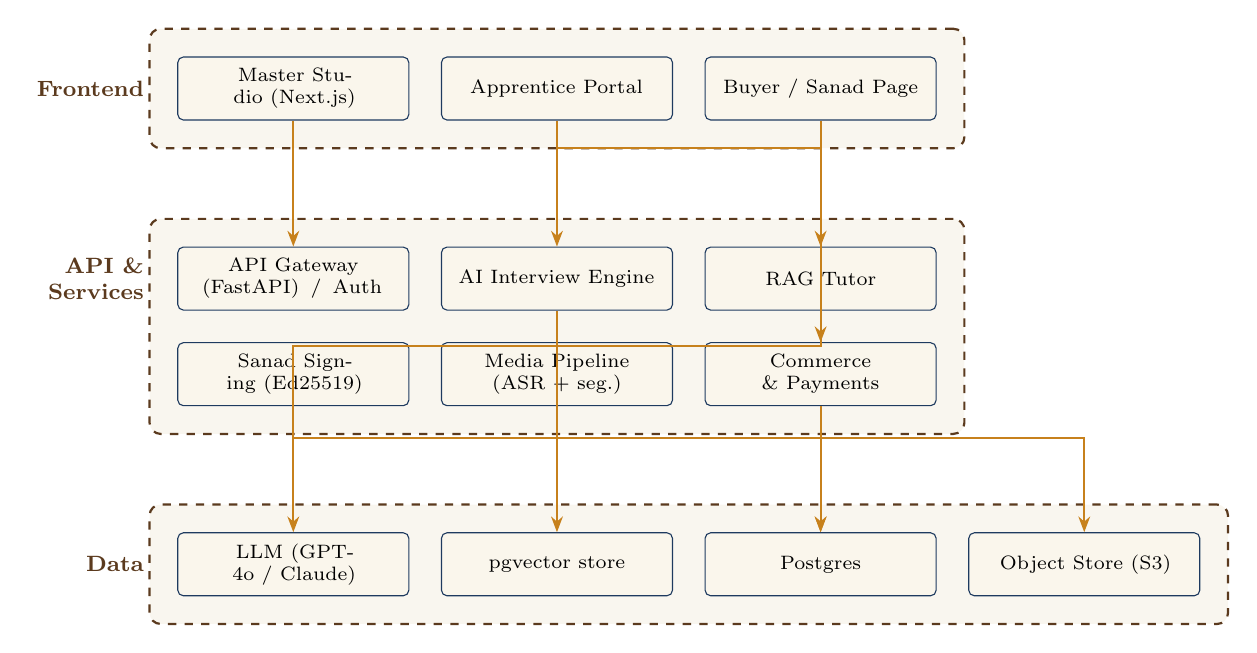
\begin{tikzpicture}[
    box/.style={rectangle, rounded corners=2pt, draw=lapis, fill=paper, text width=2.7cm, minimum height=0.8cm, align=center, font=\scriptsize},
    layerbox/.style={rectangle, rounded corners=4pt, draw=walnut, dashed, thick, fill=paperdark, fill opacity=0.35, inner sep=10pt},
    layerlabel/.style={font=\bfseries\footnotesize\color{walnut}},
    arr/.style={-{Stealth[length=2mm]}, thick, color=saffron},
  ]
  % Layer 1: Frontend
  \node[box] (master) at (0,0) {Master Studio (Next.js)};
  \node[box, right=0.4cm of master] (apprentice) {Apprentice Portal};
  \node[box, right=0.4cm of apprentice] (buyer) {Buyer / Sanad Page};
  \node[layerlabel, left=0.3cm of master] {Frontend};
  \begin{scope}[on background layer]
    \node[layerbox, fit=(master)(apprentice)(buyer)] {};
  \end{scope}

  % Layer 2: API + Services
  \node[box, below=1.6cm of master] (api) {API Gateway (FastAPI) \,/\, Auth};
  \node[box, right=0.4cm of api] (interview) {AI Interview Engine};
  \node[box, right=0.4cm of interview] (rag) {RAG Tutor};
  \node[layerlabel, left=0.3cm of api, align=right] {API \&\\Services};

  \node[box, below=0.4cm of api] (sanad) {Sanad Signing (Ed25519)};
  \node[box, right=0.4cm of sanad] (media) {Media Pipeline (ASR + seg.)};
  \node[box, right=0.4cm of media] (commerce) {Commerce \& Payments};
  \begin{scope}[on background layer]
    \node[layerbox, fit=(api)(interview)(rag)(sanad)(media)(commerce)] {};
  \end{scope}

  % Layer 3: Data
  \node[box, below=1.6cm of sanad] (llm) {LLM (GPT-4o / Claude)};
  \node[box, right=0.4cm of llm] (vec) {pgvector store};
  \node[box, right=0.4cm of vec] (db) {Postgres};
  \node[box, right=0.4cm of db] (s3) {Object Store (S3)};
  \node[layerlabel, left=0.3cm of llm] {Data};
  \begin{scope}[on background layer]
    \node[layerbox, fit=(llm)(vec)(db)(s3)] {};
  \end{scope}

  % Inter-layer arrows
  \draw[arr] (master.south) -- ++(0,-0.35) -| (api.north);
  \draw[arr] (apprentice.south) -- ++(0,-0.35) -| (interview.north);
  \draw[arr] (apprentice.south) -- ++(0,-0.35) -| (rag.north);
  \draw[arr] (buyer.south) -- ++(0,-0.35) -| (commerce.north);

  \draw[arr] (interview.south) -- ++(0,-0.45) -| (llm.north);
  \draw[arr] (rag.south) -- ++(0,-0.45) -| (vec.north);
  \draw[arr] (sanad.south) -- ++(0,-0.4) -| (db.north);
  \draw[arr] (media.south) -- ++(0,-0.4) -| (s3.north);
  \draw[arr] (commerce.south) -- ++(0,-0.4) -| (db.north);
\end{tikzpicture}
\end{center}

\subsection{Stack}

\begin{center}
\small
\begin{tabularx}{\linewidth}{>{\bfseries}lX}
\toprule
Layer & Choice \\
\midrule
Frontend & Next.js 14 (App Router) + TypeScript + Tailwind + shadcn/ui; i18n with next-intl (Koshur/Urdu/English) \\
Backend & FastAPI (Python) — same language as the AI/ML pipeline, fewer context switches \\
Database & Postgres + pgvector (embeddings); Drizzle or SQLAlchemy \\
Storage & S3-compatible (Cloudflare R2 or AWS S3) for video/audio \\
Auth & Clerk or Supabase Auth (phone-OTP first; Kashmiri masters have phones, not emails) \\
LLM & GPT-4o or Claude 3.5 Sonnet for interviewer + tutor; Whisper-large-v3 for ASR; AI4Bharat / Bhashini-compatible models considered for Koshur \\
Crypto & libsodium / PyNaCl for Ed25519 keypair generation, signing, verification \\
QR & qrcode (Python) on the server; rendered on the Sanad PDF and product tag \\
Payments (demo) & Stripe / Razorpay test mode \\
Hosting & Vercel (frontend), Railway / Render (backend), Cloudflare R2 (storage) \\
\bottomrule
\end{tabularx}
\end{center}

\subsection{The Koshur language problem and how we handle it}

Koshur ASR quality is genuinely uneven. Our fallback ladder, in priority order:

\begin{enumerate}
  \item Try AI4Bharat / Bhashini Koshur ASR if available
  \item Fall back to Urdu ASR (Koshur written in nastaliq is largely intelligible to Urdu models)
  \item Fall back to manual on-screen transcription correction (the facilitator types as the master speaks; this is acceptable in a Master Studio session and ensures perfect ground truth)
\end{enumerate}

We never let bad transcription pollute the corpus. Every Master Studio transcript is human-reviewed before it enters the Academy index.

\subsection{Why this is genuinely hard (and worth a hackathon prize)}

\begin{itemize}
  \item Multi-modal capture pipeline — synchronised voice + video + structured prompts in low-bandwidth conditions
  \item Domain-specific RAG — generic LLMs do not know craft terms; we build a Kashmiri craft vocabulary layer
  \item Structured extraction — turning unstructured Koshur speech into a typed technique knowledge graph requires careful prompt engineering and schema validation
  \item Cryptographic provenance — the Sanad is not a sticker; it is a verifiable signature anyone can check offline
  \item Voice-first UX for low-literacy elderly users — almost no tech product is genuinely designed for a 70-year-old non-Anglophone master
\end{itemize}

% =============================================================================
\section{Team \& Work Distribution (5 people, 2 + 2 + 1)}
% =============================================================================

The team is divided into three tracks. Tracks A and B run in parallel; the Lead Track owns everything where AI judgement and cryptography meet.

\begin{center}
\small
\begin{tabularx}{\linewidth}{>{\bfseries}lXX}
\toprule
Track & Composition & Scope \\
\midrule
Lead (L) & 1 person & The AI core + cryptographic Sanad + final demo orchestration \\
Track A & 2 people & Backend, data, infrastructure, payments \\
Track B & 2 people & Frontend, UX, design, pitch \\
\bottomrule
\end{tabularx}
\end{center}

\subsection{Lead Track (L) — AI Core \& Cryptographic Sanad}

\begin{itemize}
  \item Design and ship the {\bfseries AI Interview Engine}: prompt architecture, structured-output schema, follow-up logic, multi-pass interview flow, schema validation
  \item Build the {\bfseries RAG pipeline} for ``Ask the Master'': transcript chunking, embeddings, retrieval with citation back to exact video timestamps, refusal-to-hallucinate guardrails
  \item Define the {\bfseries Digital Talim schema} (technique graph, lineage, materials, failure modes) and the LLM-driven extractor that produces it from raw transcripts
  \item Integrate {\bfseries ASR} (Whisper + Koshur/Urdu fallback ladder) and translation
  \item Build the {\bfseries Sanad signing service}: Ed25519 keypair lifecycle, metadata canonicalisation, signing, public verification endpoint, QR payload format
  \item Own the {\bfseries demo dry-runs} the day before; act as on-stage operator during pitch
\end{itemize}

\subsection{Track A — Platform, Data \& Commerce (2 people)}

\textbf{Person A1 — Backend \& Data}
\begin{itemize}
  \item FastAPI service skeleton, auth, request validation
  \item Postgres schema (Master, Talim, Lesson, Learner, Sanad, Order); migrations
  \item pgvector setup, embedding storage, retrieval API
  \item Object storage integration: signed upload URLs for video/audio; chunked uploads
  \item Media pipeline: video segmentation, thumbnailing, ASR job queue
\end{itemize}

\textbf{Person A2 — Sanad Service, Commerce \& Deployment}
\begin{itemize}
  \item Public Sanad provenance page (server-rendered, no JS required to verify)
  \item QR generation, scan-event analytics
  \item Storefront checkout: Stripe / Razorpay test integration, order recording, artisan payout split
  \item DevOps: Vercel + Railway / Render deployment, environment management, basic CI
  \item Seeds, fixtures, demo data scripts so the demo can be reset cleanly
\end{itemize}

\subsection{Track B — Frontend, UX \& Pitch (2 people)}

\textbf{Person B1 — Master Studio \& Apprentice Portal}
\begin{itemize}
  \item Master Studio UI: voice-first onboarding, large-tap targets, Koshur locale, recording widget, real-time transcript view, on-screen transcript correction
  \item Apprentice Portal: lesson player with timestamped chapters, progress tracker, AI tutor chat with citation playback, practice submission flow
  \item Component library, design system (Kashmir-rooted palette and typography)
\end{itemize}

\textbf{Person B2 — Buyer Experience, Brand \& Pitch}
\begin{itemize}
  \item Public Sanad / provenance page UX (auto-translated, mobile-first)
  \item Marketing landing page; Verified Successor lineage explorer
  \item Brand identity: logo, type, motifs (drawing on talim notation aesthetics)
  \item Pitch deck (12--14 slides) and demo storyboard; rehearses the on-stage script with the Lead
  \item Ideally: arrange one short field interaction with a real artisan during build, even a 30-minute call, to validate the Master Studio flow
\end{itemize}

\subsection{Cross-track agreements (signed on day 1)}

\begin{itemize}
  \item \textbf{Schema contracts.} L locks the Digital Talim and Sanad payload schemas before A and B start integrating. No schema changes after the lock without a 15-minute team meeting.
  \item \textbf{Vertical slice first.} On day 1, the team ships the most boring possible end-to-end path (record $\to$ store $\to$ list $\to$ play $\to$ sign $\to$ verify) before adding any AI. The AI is layered on top of a working pipe.
  \item \textbf{Demo freeze 6 hours before pitch.} No code changes after freeze. Only demo rehearsal, asset prep, and pitch polish.
\end{itemize}

% =============================================================================
\section{Build Plan — Phased Within The Hackathon Window}
% =============================================================================

We assume a typical hackathon window. Phases are sequenced by dependency, not by clock-hours, so the team can compress or extend depending on the actual format.

\begin{center}
\small
\begin{tabularx}{\linewidth}{>{\bfseries}lXX}
\toprule
Phase & Work & Owner(s) \\
\midrule
P0 — Setup & Repo, branch protection, env keys, baseline schemas, deployment skeletons & A1, A2 \\
P1 — Vertical slice & Record audio in Master Studio $\to$ store $\to$ playback in Apprentice $\to$ sign Sanad $\to$ verify; no AI yet & B1 + A1 + L \\
P2 — AI Interview & Prompt + schema for structured Master Studio interview; Koshur transcript and translation & L \\
P3 — RAG tutor & Embed transcripts; retrieval; citation; refusal logic & L \\
P4 — UX polish & Master Studio recording UX; Apprentice lesson player; tutor chat UI & B1, B2 \\
P5 — Sanad \& commerce & Public provenance page; QR; Stripe / Razorpay test; lineage explorer & A2, B2 \\
P6 — Demo dataset & Record (or stage) one Sozni master session end-to-end; capture jury demo assets & L + B2 \\
P7 — Demo freeze \& rehearsal & Three full-run rehearsals; offline asset cache; failure-mode rehearsal (what if Wi-Fi dies?) & All \\
\bottomrule
\end{tabularx}
\end{center}

% =============================================================================
\section{Risks \& Mitigations}
% =============================================================================

\begin{center}
\small
\begin{tabularx}{\linewidth}{>{\bfseries}lXX}
\toprule
Risk & Likelihood & Mitigation \\
\midrule
Koshur ASR is unreliable & High & Three-tier fallback (Koshur $\to$ Urdu $\to$ manual). Demo uses pre-corrected transcript. \\
LLM tutor hallucinates a craft fact & Medium & Strict RAG: tutor must cite a video timestamp; refuses if no source. Pre-loaded craft vocabulary. \\
No real master available for hackathon recording & Medium & Pre-arrange one CDI Srinagar / family-network artisan; if all fails, a team member who has trained in sozni acts as informant for a demo-only session, clearly labelled. \\
Demo Wi-Fi fails on stage & High & All assets cached locally; LLM responses pre-recorded for the exact demo questions; offline verification of Sanad signature is a live demo. \\
Scope creep into workshops / marketplace & High & Out-of-scope list above is final. Team lead has authority to reject during build. \\
Cultural insensitivity in AI prompts & Medium & Every interview-prompt set reviewed by a Kashmiri team member or external Kashmiri advisor before shipping. \\
\bottomrule
\end{tabularx}
\end{center}

% =============================================================================
\section{Why TALIM, Why Now, Why Kashmir}
% =============================================================================

\begin{kashmirbox}[For the jury at NIT Srinagar]
This is the first generation in 400 years of Kashmiri craft history that has the technological means to capture a master's complete knowledge before they pass. It is also the first generation in 400 years where most masters' children will not enter the workshop. These two facts collide in this decade.\\[5pt]
TALIM exists because we believe Kashmir's crafts deserve the same permanent infrastructure that the rest of the world's institutional knowledge has. A scientific paper survives. A patent survives. A line of code in a public repository survives. A 400-year-old sozni stitch held only in one elderly man's hands does not. We are building so that it does.\\[5pt]
We are also building this in Srinagar, with Srinagar institutions, in service of Srinagar artisans first. The world expansion comes later. The first 100 Digital Talims will be Kashmiri. The corpus will be opened, with masters' consent, to NIT Srinagar researchers, CDI students, and recognised guilds. Whatever else this becomes, it begins here, on purpose.
\end{kashmirbox}

\subsection{What we will ask the jury for, beyond a prize}

\begin{itemize}
  \item One faculty mentor at NIT Srinagar to advise the technical roadmap
  \item An introduction to one master at the Crafts Development Institute, Srinagar, for the first real Master Studio recording
  \item A letter of support to apply for J\&K Handicrafts \& Handloom Department pilot funding
\end{itemize}

A win is not the end. It is the moment we earn the right to record the first 100 masters before more of them pass.

% =============================================================================
\section{Closing — Sixty-Second Jury Pitch}
% =============================================================================

\begin{insightbox}[If the jury asks for one minute]
\textbf{The problem:} Kashmir's master craftsmen are dying, and their children are not learning the craft, because middlemen take 80\% of every shawl's value and there is no way to learn a stitch from a master who lives three valleys away. When the master goes, the stitch goes.\\[5pt]
\textbf{The solution:} TALIM. We sit with each master in their own workshop, record an AI-led interview in Koshur, and produce a Digital Talim — a structured, multilingual, queryable record of every technique they know. Anyone can then learn from that master through the TALIM Academy with an AI tutor that cites the master's own words and clips. Every authentic piece is signed with a cryptographic Sanad, sold direct, and the artisan keeps 94\%.\\[5pt]
\textbf{The name:} The {\itshape talim} is the encoded weaving notation Kashmiri masters invented centuries ago to teach apprentices they had never met. We did not invent this idea. They did. We are building its digital, AI-native form.\\[5pt]
\textbf{The moat:} Every recording is irreplaceable. The first interviews enter the canonical Kashmiri craft corpus permanently. Every year we wait, more knowledge is lost forever.\\[5pt]
\textbf{The ask:} Help us record the first 100 masters before they are gone.
\end{insightbox}

\smallskip

\begin{warnbox}
\textbf{The truth this hackathon needs to acknowledge:} this work is genuinely racing biology. There is no software-engineering version of this problem where waiting a year is fine. Every season that passes, an {\itshape ustaad} dies somewhere in Srinagar, Pampore, Kanihama, or Sopore, and a stitch goes with him. TALIM is not an app idea. It is a form of cultural triage. We are asking to be allowed to start.
\end{warnbox}

\vspace{0.6em}

\noindent\color{rule}\rule{\linewidth}{1pt}

\begin{center}
\small\color{muted}
\textbf{TALIM} \;\textbar\; Digital Apprenticeship for Kashmir's Living Crafts \;\textbar\; Hackathon Pitch \;\textbar\; 2025\\[3pt]
\itshape The talim is what is written. The stitch is what continues.
\end{center}

\end{document}
